\newcommand{\CLASSINPUTinnersidemargin}{1.5cm}
% TODO: Check correct class
\documentclass[conference]{IEEEtran}
\IEEEoverridecommandlockouts
% The preceding line is only needed to identify funding in the first footnote. If that is unneeded, please comment it out.

%% PACKAGES
\usepackage{lipsum}   % TODO: Remove once unused
\usepackage{easyReview2}
\usepackage{multirow}
\usepackage{amsmath}
\usepackage{multicol}
\usepackage{balance}
\usepackage{graphicx}
\usepackage{minted}
\setminted[]{
    frame=lines,
    numbersep=5pt,
    breaklines,
    fontsize=\small,
    xleftmargin=.2cm
}


\graphicspath{{img/}}

\begin{document}

% TODO: Title
% ARTICLE TITLE
\title{Title}

% TODO: Authors
% AUTHORS
\author{
\IEEEauthorblockN{Author 1}
\IEEEauthorblockA{\textit{Laboratoire Lab-STICC} \\
\textit{ENSTA Bretagne}\\
29200 Brest, France \\
email@author1.org}
\and
\IEEEauthorblockN{Author 2}
\IEEEauthorblockA{\textit{Laboratoire Lab-STICC} \\
\textit{ENSTA Bretagne}\\
29200 Brest, France \\
email@author2.org}
}

\maketitle

%% The abstract is a short summary of the work to be presented in the
%% article.
\begin{abstract}



\end{abstract}



% TODO: Keywords
\begin{IEEEkeywords}
KW1, KW2
\end{IEEEkeywords}

% ==============================================
% Introduction:
% - Context
% - Presentation of the solution
% - Contributions
% - Sections
% ==============================================

\section{Introduction}

\lipsum[1]

Cite works like \cite{confexample,journalexample,presexample,techreportexample,bookexample}.

% ==============================================
% Background:
% - 
% - 
% - 
% ==============================================

\section{Background - }

\lipsum[3]

\begin{figure}[htbp]
	\centering	
	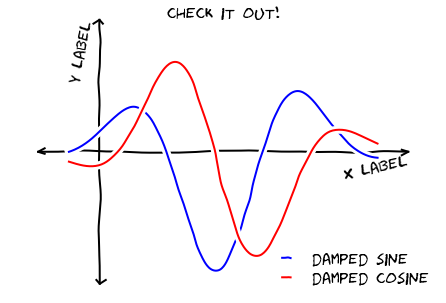
\includegraphics[width=0.48\textwidth]{default.png}
	\caption[Default Small Caption]{Default Caption.}
	\label{fig:DefaultLabel}
\end{figure}

\lipsum[4]

% ==============================================
% Related Works:
% - 
% - 
% - 
% ==============================================

\section{Related Works - }

\lipsum[5]

%           [options] {language}        {file}
\inputminted[linenos]{javascript}{codes/example.js}

% ==============================================
% Solution Design:
% - 
% - 
% -
% ==============================================

\section{Solution Design}

\lipsum[6]

% =========================================================================================
% Gigue parameters
\begin{table}[htbp]
\centering
\begin{tabular}{lll}
\hline
\textbf{Type} & \textbf{Description} & \textbf{Name} \\ \hline
\textit{1} & Param type 1 & \texttt{p1} \\ \hline
\textit{1} & Param type 2 & \texttt{p2} \\ \hline
\textit{1} & Param type 3 & \texttt{p3} \\ \hline
\end{tabular}
\caption{Table name.}
\label{tab:param}
\end{table}
% =========================================================================================

% ==============================================
% Evaluation:
% - 
% - 
% -
% ==============================================

\section{Evaluation}

\subsection{Experimental Setup}

\lipsum[7]

\subsection{Results}

\lipsum[8]

\subsection{Discussion}

\lipsum[9]

% ==============================================
% Conclusion
% - Contrib recap
% - Results recap
% - Future Works
% ==============================================

\section{Conclusion}

\lipsum[10]


\balance
\nocite{*}
\bibliographystyle{IEEEtran}
\bibliography{bibliography}


\end{document}
